\documentclass{article}
\usepackage[utf8]{inputenc}
\usepackage[T1]{fontenc}
\usepackage{graphicx}
\usepackage{float}
\begin{document}

\section*{Slide 1}

Journal of 
Instrumentation

You may also like

PAPER   OPEN ACCESS

-

The new front-end electronics for the 
ATLAS Tile Calorimeter Phase 2 Upgrade 
A. Gomes

Radiation studies performed on the High 
Luminosity ATLAS TileCal link Daughterboard

-

A prototype for the upgraded readout 
electronics of TileCal 
D Eriksson, S Muschter, K Anderson et al.

To cite this article: E. Valdes Santurio et al 2023 JINST 18 C04011

-

A radiation tolerant Data link board for the 
ATLAS Tile Cal upgrade 
H. Akerstedt, C. Bohm, S. Muschter et al.

View the  article online  for updates and enhancements.

This content was downloaded from IP address 194.12.189.145 on 09/06/2026 at 00:15

\section*{Slide 2}

Published by IOP Publishing for Sissa Medialab

Received:   October 17, 2022 
Revised:   January 22, 2023 
Accepted:   March 3, 2023 
Published:   April 20, 2023

Topical Workshop on Electronics for Particle Physics 
Bergen, Norway 
19--23 September 2022

2023 JINST 18 C04011

Radiation studies performed on the High Luminosity

ATLAS TileCal link Daughterboard

E. Valdes Santurio, * S. Silverstein,   C. Bohm,   H. Motzkau,   C. Clement,   K. Dunne   and S. Lee

on behalf of the ATLAS Tile Calorimeter System

Fysikum, Stockholm University, 
Roslagstullsbacken 21, Stockholm, Sweden

E-mail:  eduardo.valdes@fysik.su.se

Abstract:   The   new   electronics   of   the   ATLAS   Tile   Calorimeter   for   the   HL-LHC   interfaces   the 
on-detector   and   off-detector   electronics   by   means   of   a   Daughterboard.   The   Daughterboard   is 
positioned on-detector featuring commercial SFPs+, CERN GBTx ASICs, ProASIC FPGAs and 
Kintex Ultrascale FPGAs.   The design minimizes single points of failure and mitigates radiation 
damage   by   means   of   a   double   redundant   scheme,   Triple   Mode   Redundancy,   Xilinx   Soft   Error 
Mitigation IP, CRC/FEC for link data transfer, and SEL protection circuitry.   We present an updated 
summary of the TID, NIEL and SEE qualification tests, and performance studies of the Daughterboard 
revision 6 design.

Keywords:   Radiation damage to electronic components; Radiation-hard detectors; Radiation-hard 
electronics

ArXiv ePrint:   2210.08661

* Corresponding author.

c  2023 The Author(s).   Published by IOP Publishing Ltd on behalf of 
Sissa Medialab.   Original content from this work may be used under the 
terms of the  Creative Commons Attribution 4.0 licence .   Any further distribution of this 
work must maintain attribution to the author(s) and the title of the work, journal citation 
and DOI.

https://doi.org/10.1088/1748-0221/18/04/C04011

\section*{Slide 3}

Contents

1 
Introduction 
1

2 
ATLAS TileCal link Daughterboard 
2

3 
Radiation requirements for the DB6 
3

4 
Radiation tests on the DB6 
3

2023 JINST 18 C04011

5 
Conclusions 
5

1 
Introduction

The Tile Calorimeter (TileCal) is a sampling calorimeter of the ATLAS Experiment [ 1 ].   TileCal is 
in charge of identifying and measuring hadronic jets and transverse missing energy.   The TileCal 
electronics   will   be   upgraded   to   face   the   higher   radiation   levels   and   increased   rates   of   pileup   at 
the High Luminosity Large Hadron Collider (HL-LHC) [ 2 ].   The upgrade project aims to provide 
continuous digital read-out of all the TileCal with improved timing and better energy resolution. 
The off-detector electronics of the upgraded TileCal will provide digitized signals at 40 MHz 
to   the   trigger   systems   through   the   Trigger   and   Data   Acquisition   interface   (TDAQi),   while   the 
so-called Front-End Link eXchange (FELIX) system will read-out data stored in pipelines in Tile 
Preprocessors (TilePPr) at 1 MHz.   The TilePPrs will interface the on- and off-detector electronics 
through multi-Gbps optical links.   The power will be monitored and distributed to the on-detector 
electronics   by   the   Detector   Control   System   (DCS)   that   interfaces   with   the   Low   Voltage   Power 
Supplies (LVPS) in charge of distributing power to all the digital and analogue electronics, and the 
High Voltage Power Supplies that will provide high voltage to each PMT.

\begin{figure}[H]
\centering
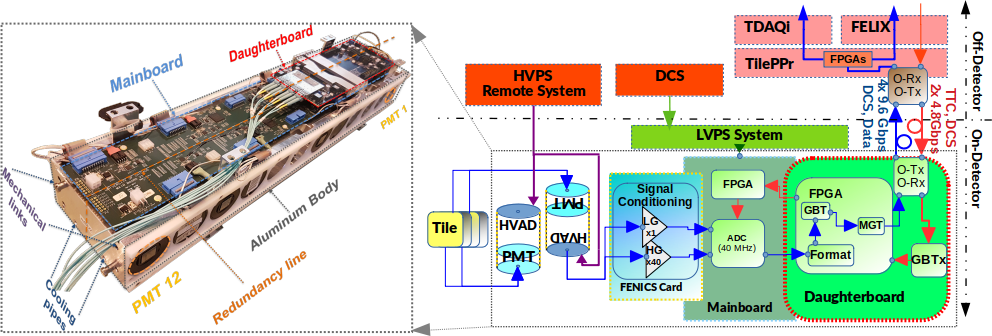
\includegraphics[width=0.8\linewidth]{assets/paper_Valdes_Santurio_2023_J._Inst._18_C04011_slide_3_item_1.png}
\end{figure}

Figure 1 .   (Left:)   TileCal Phase-II Upgrade Minidrawer.   (Right:)   On-Detector and Off-detector electronics 
block diagram.

-- 1 --

\section*{Slide 4}

The on-detector is comprised by 896 Minidrawers (MDs), in which data from all TileCal PMTs 
will continuously be sampled at 40 MHz.   Each MD (figure  1 ) will host up to twelve channels by 
means of twelve PMTs that turn light pulses to electric signals to be shaped and conditioned by 
Front-End Boards.   A Mainboard (MB) will continuously sample and digitize two gains of shaped 
signals of the MD PMTs.   A Daughterboard (DB) is in charge of distributing LHC synchronized 
timing, configuration and control to the front-end, and continuously transmitting the digital data 
from all the MB channels to the off-detector systems via multi-Gbps optical links.

2 
ATLAS TileCal link Daughterboard

2023 JINST 18 C04011

The DB is a radiation tolerant board with a redundancy layer of two functionally-equivalent halves, 
interconnecting the on- and off-detector by means of a 400-pin FMC connector and multi-Gbps 
optical links, respectively [ 3 ].   The DB, currently on its sixth revision (DB6, figure  2 ), powers the 
optical links by means of four SFP+ modules that drive two downlinks and four uplinks. 
Taking into consideration the position of the DB in ATLAS, commercial off-the-shelf components 
have been used for the design following the availability of the required components in the market, 
with the exception of the CERN radiation hard GBTx ASICs [ 4 ], due to the importance of the stable 
clock recovery and distribution very specific to the LHC readout systems.   Reported radiation tests 
studies performed in the ProASIC [ 6 ] and the Kintex Ultrascale FPGAs [ 7 ,  8 ] in addition to the 
tests performed internally in the collaboration were taken into consideration for the selection of the 
aforementioned components due to their complex nature.   The remaining part of the COTS were 
tested up the radiation requirements in parallel to the board development process.

\begin{figure}[H]
\centering
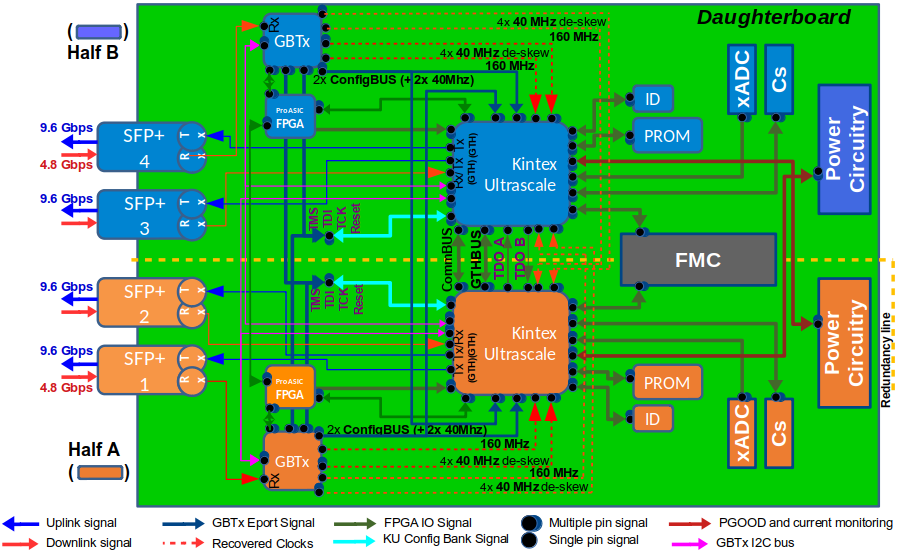
\includegraphics[width=0.8\linewidth]{assets/paper_Valdes_Santurio_2023_J._Inst._18_C04011_slide_4_item_1.png}
\end{figure}

Figure 2 .   The Daughterboard revision 6 block diagram.

The   information   received   by   the   board   from   the   off-detector   by   means   of   4.8   Gbps   GBT- 
FEC   downlinks   powered   by   CERN   radiation   hard   GBTx   ASICs   includes   clock   signals,   time

-- 2 --

\section*{Slide 5}

synchronization, and configuration commands (via the ConfigBUS path).   Two ProASIC FPGAs 
buffer   the   resets   and   JTAG   signals   (TMS,TCK   and   TDI)   received   from   the   GBTx   chips   for   the 
remote reconfiguration of the Xilinx Kintex Ultrascale (KU) FPGAs.   The two 20 nm planar featured 
KU FPGAs distribute clocks and configuration received from the GBTx to the MB, while reading 
slow integrator data and fast digitized data from two different gains of the PMTs.   The xADCs of the 
KU FPGAs sample temperature, voltage stability and currents.   Additionally, the KU FPGAs are 
connected to the Cs and xADC headers for extra digital and analog capabilities respectively, and 
communicate with each other for monitoring purposes via the so called CommBUS and GTHBUS. 
An over-current protection circuit triggers a power cycle in the case of the presence of high currents. 
Each   KU   FPGA   sends   data   off-detector   by   means   of   two   copies   of   GBT-FEC   protected   words 
through two 9.6 Gbps uplinks.   The board radiation tolerance is achieved by the redundancy layers 
in the design, using the Xilinx Soft Error Management (SEM), Triple Mode Redundancy (TMR), 
GBT-FEC protocol, and GBTx ASICs.

2023 JINST 18 C04011

3 
Radiation requirements for the DB6

The radiation levels that the DB is expected to be exposed to were calculated from the radiation 
simulations performed by the ATLAS Collaboration to estimate the expected radiation levels for 
the HL-LHC era [ 9 ].   The most irradiated positions where the DB will be installed was used as a 
reference value for the radiation requirements.   Approximately 108 Gy is the Total Ionizing Dose 
(TID) required for the design to be qualified, taking into consideration Safety Factors (SF) of 1 . 5 for 
simulation and 3 . 0 for lot variation in the components.   The Non-Ionizing Energy Losses (NIEL) 
fluence   required   is   for   qualification   is   13 . 16  $\times$  10 12   n/cm 2 ,   including   SFs   of   1 . 5   for   simulation, 
1 . 3   when   using   a   non-monoenergetic   neutron   source,   and   3 . 0   to   account   for   lot   variation   of   the 
components.   The expected fluence for Single Event Effects is 4 . 54  $\times$  10 11   h/cm 2 , where a SF = 
3 . 0   for   simulation   was   included   in   the   calculations.   All   the   aforementioned   requirement   values 
have been put into place in accordance with the ATLAS Radiation Tolerant Electronics Proposed 
Guideline on COTS Lot to Lot Variation [ 10 ].

4 
Radiation tests on the DB6

Four Daughterboards were produced and separately used to test for radiation tolerance, labelled in 
this document as DB6-0, DB6-1, DB6-2 and DB6-3. 
Two separate tests were performed to cover tolerance to TID.   The KU FPGA temperatures 
and all the currents corresponding to all the point of load regulators of the irradiated boards were 
monitored.   Special attention was placed on the total of ten Coretek SFP+, the six KU FPGAs, the 
six Microsemi ProaSIC3 FPGAs and the IS25LP128F reconfiguration FLASH memories.   None 
of the components were damaged by the deposited TID: DB6-1 and DB6-2 were irradiated with 
Gamma radiation at   60 Co at the CERN CC60 facilities to 220 Gy at a rate of 3.37 Gy/h (figure 9 of 
ref. [ 11 ]) and up to 54 Gy at a rate of 0.33 Gy/h (figure 10 of ref. [ 11 ]), respectively.   DB6-1 ran 
stable during the full test, however it showed an increase in the current measured in the 0.95 V power 
line of both sides of the board of at around 140 Gy.   This was demonstrated to be correlated with the 
failure of the active components of the fan used to keep the KU FPGAs cool, leading to the increase

-- 3 --

\section*{Slide 6}

of temperature on the FPGA.   The currents, temperatures and functionalities of the DB6-2 were 
stable during the full run.   DB6-3 was irradiated in the AlC-144 cyclotron proton beam line with 
54 MeV protons at the IFJ in Krakow to 381 Gy for half-A FPGA and 400 Gy for half-B FPGA at a 
rate of 2.88 Gy/h (figure  3 ).   All the currents and the temperatures were stable during the full run. 
The higher fluctuations compared with DB6-1 (0 to 140 Gy) and DB6-2 are due to active Single 
Event Upset (SEU) corrections by the Xilinx SEM and resets applied when an uncorrectable SEU 
appeared during the run. 
For the Single Event Latchups (SEL) tests, there was no prototype of the DB produced and the 
design was migrating from the 16 nm FinFET powered KU+ FPGA to the KU FPGA, due to the 
KU+ alternative been susceptible to SEL occurrences.   As an alternative to the ProASIC, a Lattice 
ICE40LP FPGA was also tested [ 11 ].   Two separate tests were performed for SEL, one as described 
for the DB6-3 with 54 MeV protons, where the FPGAs were irradiated to a fluence of 2 . 62  $\times$  10 11

2023 JINST 18 C04011

p/cm 2 .   In the second test, two Trenz TE0841 boards (each with the same KU FPGA used in the 
DB design), a Lattice ICE40LP FPGA and a ProASIC3E A3P31500 FPGA were irradiated with 
226 MeV protons to a fluence of 1 . 11  $\times$  10 12   p/cm 2 , for which all the currents of the FPGAs were 
monitored (figure 6 of ref. [ 11 ]).   No SEL were observed in the units under test in either of the tests.

\begin{figure}[H]
\centering
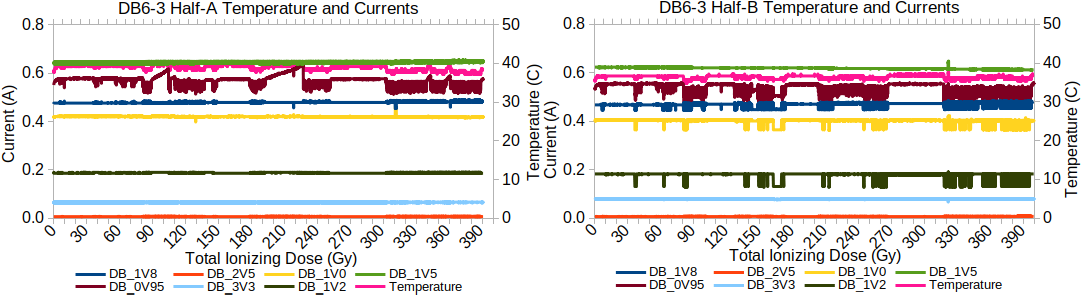
\includegraphics[width=0.8\linewidth]{assets/paper_Valdes_Santurio_2023_J._Inst._18_C04011_slide_6_item_1.png}
\end{figure}

Figure 3 .   TID test of DB6-3.   All board currents and the temperatures of both KU FPGAs were monitored 
over the whole irradiation period delivered by a 54 MeV proton beam.

A set of tests was arranged in coordination with the RIC Jozef Stefan Institute in Ljubliana, to 
cover the NIEL tolerance, where a DB (DB6-0) and a set of test boards with non-radiation qualified 
DB components were irradiated in the beam port number 6 of the TRIGA reactor [ 5 ] to a fluence of 
14  $\times$  10 12   (1 MeV equivalent n)/cm 2 .   The post-radiation tests performed on DB6-0 demonstrated the 
radiation tolerance of the KU FPGAs up to the exposed fluence.   In the case of the ProASIC, some 
after-effects could be seen where the firmware was not working as expected and re-configuration was 
not possible.   However, the firmware functionality of all devices was recovered after annealing, with 
re-configuration capability recovered all of the devices.   The same applies to the IS25LP128F FLASH 
memories, where after annealing some of the devices recovered the re-programing capabilities, with 
all the contents of the memory not being affected in any of the devices. 
Four different variants of 10 Gbps multi-mode SFP+ devices were tested:   AVAGO, CORETEK, 
FS-Europe and Direktronik.   The two AVAGO AFBR-709SMZ devices completely failed to pass 
the   irradiation   tests   done   up   to   9  $\times$  10 12   (1 MeV   equivalent   n)/cm 2   fluence.   One   out   of   nine 
CORETEK CT-A000NPP-SB1L-D devices tested failed to function after irradiating to 9  $\times$  10 12

(1 MeV   equivalent   n)/cm 2   fluence.   In   the   case   of   the   Direktronik   33-4248   and   the   FS-Europe

-- 4 --

\section*{Slide 7}

SFP-10GSR-85 devices, one of each of the two brands was exposed to a higher fluence of 14  $\times$  10 12

(1 MeV equivalent n)/cm 2 , and a batch of ten of each of the two brands was exposed to 7  $\times$  10 12

(1 MeV equivalent n)/cm 2   fluence.   All of the samples irradiated from Direktronik and FS-Europe 
were fully functional after irradiation. 
It was seen that the threshold voltages for the FDFMA3N109 MOSFETs used in the design 
shifted   with   the   exposure   (figure   4 )   due   to   the   Gamma   component   present   in   the   reactor   cavity 
(195 Gy).   The asymmetrical profile of the flux in the cavity was used to have a perception of the 
correlation between the shifts of the thresholds in the MOSFETs and the exposed fluence.   Four out 
of fifteen QUAD oscillators LTC6902IMS irradiated failed to pass the post irradiation tests, therefore 
the device needs to be removed from the design.   The rest of the components (DAN217T146CT 
Schottky diodes, 540BAA100M000BBG oscillators and INA333AIDRG instrumentation amplifiers) 
passed the post radiation tests with no issues.

2023 JINST 18 C04011

\begin{figure}[H]
\centering
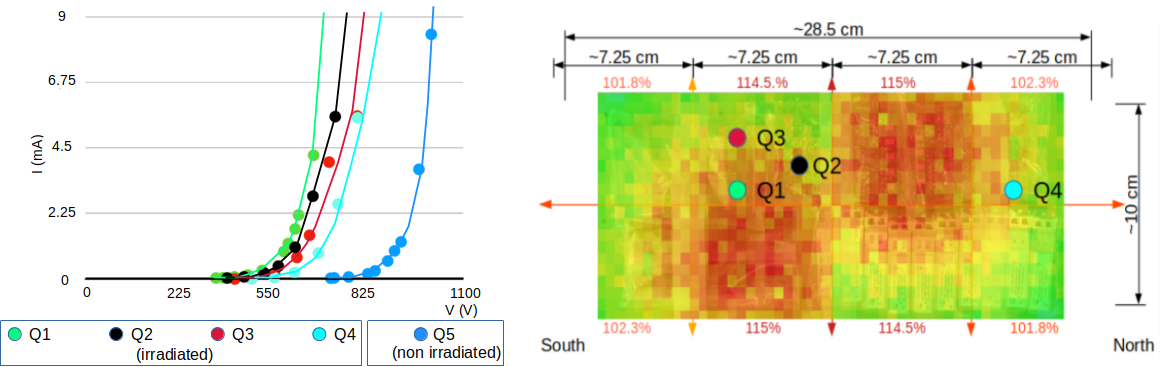
\includegraphics[width=0.8\linewidth]{assets/paper_Valdes_Santurio_2023_J._Inst._18_C04011_slide_7_item_1.png}
\end{figure}

Figure 4 .   (Left:)   Threshold shift depicted in an IV curve of four of the irradiated FDFMA3N109 MOSFETs. 
(Right:)   Position of the irradiated MOSFETs in the flux 2D slice map of the reactor cavity.

5 
Conclusions

Radiation tests were conducted to determine the suitability of each component and part of the DB6 
design for meeting HL-LHC requirements.   The results of the completed tests have demonstrated that 
the key components of the design have TID, NIEL, and SEL resistance up to the necessary radiation 
levels, with a few non-critical, radiation-sensitive parts still requiring attention.   Additional TID and 
SEL testing needs to be carried out on certain SFP+ variants. 
Some radiation sensitive parts of the features of the design need modification:

   The supplementary over-current protection circuit added for SEL mitigation has to be removed 
because of the radiation induced variations in the threshold of the FDFMA3N109 MOSFETS 
used in the design.

   The LTC6902IMS QUAD oscillators, previously used to de-couple the phase of the DC-DC 
converters, has to be removed from the design.   Further research is necessary to evaluate the 
effect of this design modification on board noise levels.

The removal of the aforementioned MOSFETs and QUAD oscillatorswill make the design components 
at a board level sufficiently resistant to the expected TID, NIEL ans SEL irradiation levels.

-- 5 --

\section*{Slide 8}

The development roadmap for the DB R\&D project includes creating additional prototypes 
incorporating   the   previously   mentioned   modifications,   conducting   SEU   tests   with   operational 
firmware to evaluate the impact of SEU rates on board performance, and analyzing test results to 
determine the final selection of the SFP+ variant that will be integrated to the final board design. 
Once the design is adjusted based on the test outcomes, prototypes will be manufactured and tested 
as part of the production phase.   The project aims to produce a total of 930 DB6 units as Stockholm 
University's contribution to the HL-LHC era for TileCal.

Acknowledgments

2023 JINST 18 C04011

This work was supported by Stockholm University and CERN.

References

[1]   ATLAS collaboration,  The ATLAS Experiment at the CERN Large Hadron Collider ,  2008  JINST   3 
S08003 .

[2]   ATLAS collaboration,  Technical Design Report for the Phase-II Upgrade of the ATLAS Tile 
Calorimeter ,  CERN-LHCC-2017-019, ATLAS-TDR-028  (2018).

[3]   E. Vald\'es Santurio,  Development of the read-out link and control board for the ATLAS Tile Calorimeter 
Upgrade , Ph.D. Thesis, Stockholm University (2019) [ISBN: 978-91-7797-896-1] 
[ http://www.diva-portal.org/smash/get/diva2:1364842/FULLTEXT03.pdf ].

[4]   K. Wyllie, P. Moreira and J. Christiansen,  GBTX MANUAL V0.15 Technical Report , (2021),

https://espace.cern.ch/GBT-Project/GBTX/Manuals/GBTXManual.pdf .

[5]   M. Ravnik,  Description of TRIGA Reactor ,

https://ric.ijs.si/wp-content/uploads/Description\_TRIGA\_Reactor.pdf .

[6]   Actel,  Radiation-Tolerant ProASIC3 FPGAs Radiation Effects , (2012),  https://www.microsemi.com/ 
document-portal/doc\_view/131374-radiation-tolerant-proasic3-fpgas-radiation-effects-report .

[7]   D.M. Hiemstra, V. Kirischian and J. Brelski,  Single Event Upset Characterization of the Zynq 
UltraScale+ MPSoC Using Proton Irradiation , in  2017 IEEE Radiation Effects Data Workshop 
(REDW) , New Orleans, LA, U.S.A. (2017), p. 1--4 [ DOI:10.1109/NSREC.2017.8115448 ].

[8]   P. Maillard, J. Barton, M.J. Hart, Y.P. Chen and M.L. Voogel,  Total Ionizing Dose and Single-Events 
characterization of Xilinx 20nm Kintex UltraScale , in  2019 19th European Conference on Radiation 
and Its Effects on Components and Systems (RADECS) , Montpellier, France (2019), p. 1--6 
[ DOI:10.1109/RADECS47380.2019.9745695 ].

[9]   ATLAS collaboration,  Radiation Environment of ATLAS ,  https://twiki.cern.ch/twiki/pub/AtlasPublic/ 
RadiationSimulationPublicResults/WebRadMaps\_Zoom\_R2\_public.html .

[10]   C. Amelung and H. Chen,  ATLAS Radiation Tolerant Electronics Proposed Guideline on COTS Lot to 
Lot Variation , (2020),  https://indico.cern.ch/event/946481/contributions/3978191/attachments/ 
2087789/3507703/COTSL2L.20200806.v2.pdf .

[11]   E. Vald\'es Santurio et al.,  R\&D Studies for the Atlas Tile Calorimeter Daughterboard ,  JACoW 
ICALEPCS2021  (2022) 290 .

-- 6 --

\end{document}
